% Канонический TikZ-рисунок варианта 16. Править только здесь.
\long\def\figStereoV16{%
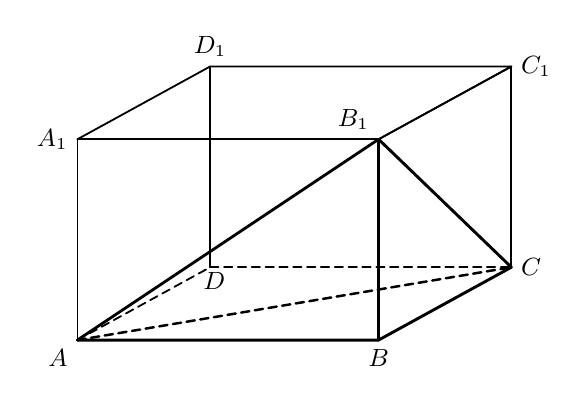
\begin{tikzpicture}[
    x={(1cm,0cm)},
    y={(0.62cm,0.34cm)},
    z={(0cm,1cm)},
    scale=0.85,
    line cap=round,
    line join=round,
    boxedge/.style={
        line width=0.65pt
    },
    hidden/.style={
        line width=0.65pt,
        dashed,
        dash pattern=on 3pt off 2pt
    },
    solid/.style={
        line width=1.05pt
    },
    solidhidden/.style={
        line width=0.9pt,
        dashed,
        dash pattern=on 3pt off 2pt
    },
    every node/.style={
        font=\small
    }
]

% =================================================
% Вершины прямоугольного параллелепипеда
% =================================================

\coordinate (A)  at (0,0,0);
\coordinate (B)  at (4.5,0,0);
\coordinate (C)  at (4.5,3.2,0);
\coordinate (D)  at (0,3.2,0);

\coordinate (A1) at (0,0,3);
\coordinate (B1) at (4.5,0,3);
\coordinate (C1) at (4.5,3.2,3);
\coordinate (D1) at (0,3.2,3);

% =================================================
% Скрытые рёбра параллелепипеда
% =================================================

\draw[hidden] (A)--(D);
\draw[hidden] (D)--(C);
\draw[hidden] (D)--(D1);

% =================================================
% Видимые рёбра параллелепипеда
% =================================================

\draw[boxedge] (A)--(A1)--(B1);
\draw[boxedge] (A1)--(D1)--(C1)--(B1);
\draw[boxedge] (D1)--(D);
\draw[boxedge] (C1)--(C);
\draw[boxedge] (B1)--(C1);

% =================================================
% Рёбра пирамиды ABCB_1
% =================================================

% Рёбра основания ABC
\draw[solid]       (A)--(B)--(C);
\draw[solidhidden] (A)--(C);

% Боковые рёбра
\draw[solid] (A)--(B1);
\draw[solid] (B)--(B1);
\draw[solid] (C)--(B1);

% =================================================
% Подписи вершин
% =================================================

\node[below left]  at (A)  {$A$};
\node[below]       at (B)  {$B$};
\node[right]       at (C)  {$C$};
\node[right, xshift=-6pt, yshift=-5pt] at (D) {$D$};

\node[left]        at (A1) {$A_1$};
\node[above left]  at (B1) {$B_1$};
\node[right]       at (C1) {$C_1$};
\node[above]       at (D1) {$D_1$};

\end{tikzpicture}
}
